\subsection{Non-Inverting Amplifier:}

Setting the {\itshape waveform generator} in a sinusoidal signal with a frequency of 1 KHz and 1 $V_{pp}$ we connect the positive terminal of the {\itshape generator} to the $V_{i}$ input of the circuit of Figure 3.2.0 ( is the op-amp terminal 3 ) \linebreak and the negative terminal to the common ground. Then, once the respectively sources in the terminals 7 and 4 were connected, we turned on the {\itshape generator} and the voltage sources, thus, connecting the channel 1 of the oscilloscope in the input $V_{i}$ and the channel 2 in the output $V_{o}$ we registered the waveform in Figure 3.2.1. \hfill \break

\begin{figure}[H]
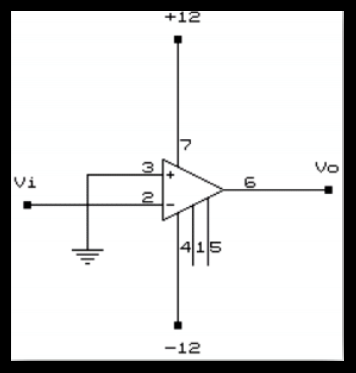
\includegraphics[width = 8cm, height = 5cm]{c2.png}
\centering \linebreak \linebreak Figure 3.2.0: Non-inverting amplifier circuit.
\end{figure} \hfill

The oscilloscope has another way to display the waveform, setting the device in its mode XY we will be able to visualize the {\bfseries Transfer Function} as in Figure 3.2.2. \hfill \break

\begin{multicols}{2}
\begin{figure}[H]
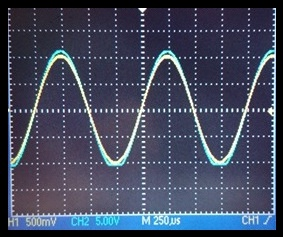
\includegraphics[width = 8cm, height = 5cm]{o2.jpg}
\centering \linebreak \linebreak Figure 3.2.1: Input and output waveform.
\end{figure}

\begin{figure}[H]
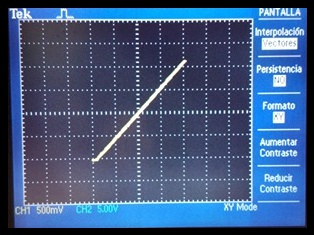
\includegraphics[width = 8cm, height = 5cm]{tf2.jpg}
\centering \linebreak \linebreak Figure 3.2.2: Transfer Function.
\end{figure}
\end{multicols} \hfill

{\bfseries\itshape\color{carmine}{Observation:}} {\itshape\color{carmine}{The yellow waveform corresponds to the channel 1 and the blue waveform to channel 2 for Figure 3.2.1.}} \hfill \break

We capture the gain and the input and output voltage values in Table 2: \hfill \break

\begin{center}
\begin{tabular}[.5cm]{c c c}
\toprule
\toprule
\hspace{60pt} $V_{i}$ \hspace{60pt} & \hspace{60pt} $V_{o}$ \hspace{60pt} & \hspace{60pt}  {\bfseries Gain} \hspace{60pt}  \\
\midrule
\midrule
1 $V_{p}$ & 10.3 $V_{p}$ & 10 \\
\bottomrule
\linebreak
\end{tabular}
\linebreak Table 2: Gain of Inverting Amplifier.
\end{center} 

\pagebreak

Finally, increasing the amplitude of the input signal we visualize that the output starts to get saturated from values bigger than 2 $V_{pp}$: \hfill \break

\begin{center}
\begin{tabular}[.5cm]{c c}
\toprule
\toprule
\hspace{85pt} $V_{sat}$ ( + ) \hspace{85pt} & \hspace{85pt} $V_{sat}$ ( - ) \hspace{85pt} \\
\midrule
\midrule
$V_{sat}\ > 1\ V_{p}$ & $V_{sat}\ < -1\ V_{p}$ \\
\bottomrule
\linebreak
\end{tabular}
\linebreak Table 3: Output saturation.
\end{center} \hfill

When the output begins to get saturated, in the oscilloscope we visualize that the output turns from a sinusoidal into a square waveform as in Figure 3.2.4: \hfill \break

\begin{figure}[H]
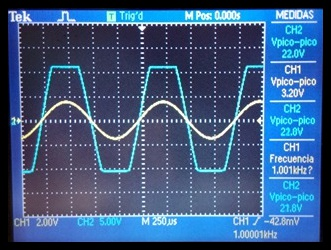
\includegraphics[width = 8cm, height = 5cm]{s1.jpg}
\centering \linebreak \linebreak Figure 3.2.4: Saturated output waveform.
\end{figure}

\pagebreak